\documentclass[usenames,dvipsnames, handout]{beamer}
\usetheme{Boadilla}
\usepackage{graphicx}
\usepackage{soul}
\usepackage{multirow}
\usepackage{multicol}
\usepackage{csvsimple}


\newcommand{\R}{\mathbb{R}}
\newcommand{\ubar}[1]{\underaccent{\bar}{#1}}
\newcommand{\Int}{\text{Int}}
\newcommand{\xbf}{\mathbf{x}}
\newcommand{\Abf}{\mathbf{A}}
\newcommand{\Bbf}{\mathbf{B}}
\newcommand{\Gbf}{\mathbf{G}}
\newcommand{\bbf}{\mathbf{b}}
\newcommand{\Lfn}{\mathcal{L}}
\newcommand{\one}{\mathbbm{1}}

\title[HW (2007)]{``How Costly is External Financing? Evidence from a Structural Estimation"\\Christopher A. Hennessy and Toni M. Whited (2007)\\Journal of Finance}
\author{Alex von Hafften}
\institute{UW-Madison}

\begin{document}

\begin{frame}
\titlepage
\end{frame}

\section{Introduction}

\begin{frame}
\frametitle{Motivation}
\small
\begin{itemize}
\item Modigliani-Miller Irrelevance Theorem (1958, 1963) 

\bigskip

\textit{In frictionless world, financing decisions like capital structure (debt vs. equity), payout policy, cash holding, etc. do not matter.}
\bigskip
\item Why? No arbitrage
\bigskip
\item MM assumes there are no financial friction:
\begin{itemize}
\item Perfect and complete capital markets
\item No taxes
\item Bankruptcy is not costly
\item Capital structure does not affect investment policy or cash flows
\item Symmetric information
\end{itemize}
\end{itemize}
\end{frame}



\begin{frame}
\frametitle{Hennessy and Whited (2007)}
\small
\begin{itemize}
\item HW (2007) formulate a dynamic structural model of optimal financial and investment policy for a firm facing
\begin{itemize}
\item Corporate and personal taxes
\item Bankruptcy costs
\item Costs to issue external equity
\end{itemize}
\bigskip
\item HW (2007) estimate parameters describing production technology and financial frictions using simulated method of moments (SMM)
\bigskip
\item HW (2007) is seminal paper that uses SMM in corporate finance
\end{itemize}
\end{frame}

\AtBeginSection[ ]
{
\begin{frame}{Outline}
    \tableofcontents[currentsection]
\end{frame}
}

\section{Model}

\begin{frame}
\frametitle{Environment - Production and Debt}
\small
\begin{itemize}
\item Estimated parameters in {\color{red}red}
\item Firm produces with $k$ capital
\item Productivity follows discretized AR(1) process in logs: 

$$
\ln z' = {\color{red}\rho} \ln z + {\color{red}\sigma_\varepsilon} \varepsilon
$$

where $\varepsilon \sim N(0, 1)$. Tauchen discretization $\implies Q(z, z')$ transition probability and finite min/max
\item Operating profits are $z k^{\color{red}\alpha}$ where ${\color{red}\alpha} \in (0, 1)$
\item Firm also has $b$ net debt
\begin{itemize}
\item $b > 0$ is one-period defaultable debt with interest rate $\tilde r$ that depends on $k$, $b$, and $z$ (not contingent on $z'$)
\item $b \le 0$ is cash that returns risk-free rate $r$
\end{itemize}

\item Firm defaults on debt if continuation value is negative
\end{itemize}
\end{frame}

\begin{frame}
\frametitle{Environment - Taxes and Equity Issuance}
\small
\begin{itemize}
\item Personal tax rate $\tau_i \implies$ firms discounts using $\frac{1}{1 + r(1-\tau_i)}$
\item Corporate taxable income is operating profits net of depreciation and interest:
$$
y \equiv z k^\alpha - \delta k - \tilde r(k, b, z^-) b
$$
\item Corporate tax schedule has ``kink" around zero
$$
T^C(y) \equiv 
\begin{cases} 
\tau_c^+ y, & \text{if }y > 0 \\
\tau_c^- y, & \text{if }y \le 0
\end{cases}
$$
\item Shareholder tax liability on dividend:
$$
T^d(div) = \int_0^{div} \tau_d(x) dx \text{ where } \tau_d(x) \equiv \bar \tau_d * [1 - e^{-{\color{red}\phi} x}]
$$
\item Firm pays fixed, linear, and quadratic costs for external equity issuance:
$$
\Lambda(iss) \equiv 
\begin{cases} 
{\color{red}\lambda_0} + {\color{red}\lambda_1} iss + {\color{red}\lambda_2} iss^2, & \text{if }iss > 0 \\
0, & \text{if }iss \le 0
\end{cases}
$$
\end{itemize}
\end{frame}



\begin{frame}
\frametitle{``Naive" Way to Write Firm Value Function}
\scriptsize
\begin{align*}
V(k, b, z, z^-) =
\max_{(k', b')} \Bigg\{ 
& \underbrace{w + b' - k'}_{\text{cash dividend } (+) \text{ or equity issuance } (-)} - \underbrace{T^d(w + b' - k')}_{\text{taxes on cash dividend}} - \underbrace{\Lambda(-(w + b' - k'))}_{\text{equity issuance cost}} \\
&+ \frac{1}{1+r(1-\tau_i)} E\Big[\underbrace{\max\{ V(k', b', z', z), 0\}}_{\text{if }V(\cdot) \text{ is } (-) \implies\text{ default}}\Big] \Bigg\} \\
\text{where }
\underbrace{y}_{\text{taxable corporate income}} &\equiv \underbrace{z k^\alpha}_{\text{operating profits}} - \underbrace{\delta k}_{\text{depreciation}} - \underbrace{\tilde r(k, b, z^-) b}_{\text{interest on debt}} \\
\underbrace{w}_{\text{realized net worth}} &\equiv \underbrace{y - T^C(y)}_{\text{after-tax corporate income}}+ \underbrace{k}_{\text{capital}}  - \underbrace{b}_{\text{debt principal}} 
\end{align*}
\end{frame}


\begin{frame}
\frametitle{Smarter Way to Write Firm Value Function}
\scriptsize
\begin{align*}
V(w, z) =
\max_{(k', b')} \Bigg\{ 
& \underbrace{w + b' - k'}_{\text{cash dividend } (+) \text{ or equity issuance } (-)} - \underbrace{T^d(w + b' - k')}_{\text{taxes on cash dividend}} - \underbrace{\Lambda(-(w + b' - k'))}_{\text{equity issuance cost}} \\
&+ \frac{1}{1+r(1-\tau_i)} E\Big[\underbrace{\max\{ V(w', z'), 0\}}_{\text{if }V \text{ is } (-) \text{ can default}}\Big] \Bigg\} \\
\text{where }
\underbrace{y'}_{\text{taxable corporate income}} &\equiv \underbrace{z' (k')^\alpha}_{\text{operating profits}} - \underbrace{\delta k'}_{\text{depreciation}} - \underbrace{\tilde r(k', b', z) b'}_{\text{interest on debt}} \\
\underbrace{w'}_{\text{realized net worth}} &\equiv \underbrace{y' - T^C(y')}_{\text{after-tax corporate income}}+ \underbrace{k'}_{\text{capital}}  - \underbrace{b'}_{\text{debt principal}} \end{align*}
\end{frame}


\begin{frame}
\frametitle{Default and Interest Rates}
\small
\begin{itemize}
\item Firm defaults on debt if $w$ below $z'$-specific threshold:
$$
\underline{w}(z') = V^{-1}(0, z') < 0 \implies z_d(k', b', z) \text{ threshold}
$$
\item If firm defaults, outside investor gets recovery value
\begin{align*}
R(k', z') &= \underbrace{(1-{\color{red}\xi}) (1-\delta)k'}_{\text{depreciated capital net of deadweight bankruptcy cost}} + \underbrace{z'(k')^\alpha}_{\text{operating profit}} \\&- \underbrace{T_c(z'(k')^\alpha - \delta k')}_{\text{corporate tax bill }} - \underbrace{\underline w (z')}_{\text{going-concern}}
\end{align*}
\item Interest rates on debt determined by zero-profit condition for outside investor
\begin{align*}
\underbrace{(1+r(1-\tau_i))b'}_{\text{risk-free investment}} 
&=
\underbrace{(1+(1-\tau_i)\tilde r(k', b', z))b' \int_{z_d(k', b', z)}^{\bar z} Q(z,dz')}_{\text{return on non-defaulted debt}} \\
&+ \underbrace{\int_{\underline z}^{z_d (k', b', z)} R(k', z') Q(z, dz')}_{\text{return on defaulted debt}}
\end{align*}
\end{itemize}
\end{frame}


\begin{frame}
\frametitle{Computation}
\small
\begin{itemize}
\item No closed form solution $\implies$ solve numerically
\bigskip
\item Computational strategy:
\begin{itemize}
\item Guess $\tilde r (k', b', z) = r$
\item Solve $V$ with value function iteration
\item Compute $z_d(k', b', z)$
\item Update $\tilde r(k', b', z)$ using zero-profit condition
\item Repeat until convergence
\end{itemize}
\end{itemize}
\end{frame}


\section{Estimation}

\begin{frame}
\frametitle{External Parameters from Related Literature}
\small
\begin{center}
\begin{tabular}{ cc } 
 \hline
 Parameter    & Value \\ 
 \hline
 $\bar\tau_d$ & 0.12 \\ 
 $\tau_i$     & 0.29 \\ 
 $\tau_c^+$   & 0.40 \\ 
 $\tau_c^-$   & 0.20 \\ 
 $r$          & 0.025 \\
 $\delta$     & 0.15 \\
 \hline 
\end{tabular}
\end{center}
\begin{itemize}
\item Notice $\tau_c^+ > \tau_c^- \implies$ corporate taxes larger on positive income than rebate for corporate losses 
\end{itemize}
\end{frame}


\begin{frame}
\frametitle{Moments Selection}
\scriptsize
\begin{center}
\begin{tabular}{ lll } 
 \hline
 Parameter            & Description & Moments \\ 
 \hline
 $\alpha$             & Profit fn. curvature  & Var. of investment \\ 
 $\lambda_i$          & Ex. equity iss. costs & Freq. negative debt \\ 
                      &                       &  Cov. equity iss. and inv. \\ 
 $\lambda_0$          & Fixed cost &Freq. and mean equity iss. \\ 
 $\lambda_2$          & Quadratic cost &Var. of equity iss. \\ 
 $\xi$                & Bankruptcy deadweight cost & Mean net debt-to-assets \\
                      &                            & Cov. of lev. and inv.\\
 $\phi$               & Shareholder tax liab. curvature & Payout ratio \\
                      &                                 & Var. of dividends \\
 $\sigma_\varepsilon$ & Productivity shock var. & SD of shock to inc.-to-assets \\
 $\rho$               & Productivity persistence & Serial cor. of inc.-to-assets \\
 \hline 
\end{tabular}
\end{center}
\begin{itemize}
\item High $\lambda_0 \implies$ fewer larger equity issuances
\item Freq. negative debt $\implies$ precautionary motion for saving
\item Cov. of equity iss. and investment informs about equity position in pecking order
\item Cov. of lev. and investment informs about debt position in pecking order 

\end{itemize}
\end{frame}

\begin{frame}
\frametitle{Moments and Estimated Parameters using SMM}
\scriptsize
\begin{center}
\begin{tabular}{ ccc } 
 \hline
 Parameter            & Estimates (HW) & SE (HW) \\ 
 \hline
 $\alpha$             & 0.627 &(0.219) \\ 
 $\lambda_0$          & 0.598 &(0.233) \\ 
 $\lambda_1$          & 0.091 &(0.026) \\ 
 $\lambda_2$          & 0.0004 &(0.0008) \\ 
 $\xi$                & 0.104 &(0.059) \\
 $\phi$               & 0.732 &(0.844) \\
 $\sigma_\varepsilon$ & 0.118 &(0.042) \\
 $\rho$               & 0.684 &(0.349) \\
 \hline 
\end{tabular}
\end{center}

\begin{center}
\csvautotabular{table_hw.csv}
\end{center}

\begin{itemize}
\item Good fit, but biggest problem is overestimate of variance of dividends (consistent with lit.)
\end{itemize}
\end{frame}

\section{Replication}


\begin{frame}
\frametitle{Replication Issues}
\scriptsize
\begin{enumerate}
\item Discount bond prices are bounded whereas interest rates are not:
\scriptsize
\begin{align*}
V(w, z) =
\max_{(k', b')} \Bigg\{ 
& \underbrace{w + b'q(k',b',z) - k'}_{\text{dividend if } (+) \text{ or equity issuance if } (-)} - \underbrace{T^d(w + b'q(k',b',z) - k')}_{\text{taxes on dividend}} \\
- &\underbrace{\Lambda(-(w + b'q(k',b',z) - k'))}_{\text{equity issuance cost}} + \frac{1}{1+r(1-\tau_i)} E\Big[\underbrace{\max\{ V(w', z'), 0\}}_{\text{if }V \text{ is } (-) \text{, default}}| z\Big] \Bigg\} \\
\text{where }
\underbrace{y'}_{\text{taxable income}} &\equiv \underbrace{z' (k')^\alpha}_{\text{operating profits}} - \underbrace{\delta k'}_{\text{depreciation}} - \underbrace{(1-q(k',b',z)) b'}_{\text{interest on debt}} \\
\underbrace{w'}_{\text{realized net worth}} &\equiv \underbrace{y' - T^C(y')}_{\text{after-tax corporate income}}+ \underbrace{k'}_{\text{capital}}  - \underbrace{q(k',b',z)b'}_{\text{debt principal}}
\end{align*}
\small
\item What is the $w$ grid?
\begin{itemize}
\scriptsize
\item HW (2007) are specific about $z$, $b$, $k$ grids, but quiet about the $w$ grid
\item My solution: Loop over $z$, $b$, $k$ grids and solve $w$ for $q = 0$ and $q = 1/(1+r)$, then linear interpolate between min and max
\end{itemize}
\item No contraction mapping for bond prices $\implies$ update $q$ guess slowly
\item Compustat data revisions
\item Unclear data appendix: number of obs. were either 2x or 0.5x
\end{enumerate}
\end{frame}



\begin{frame}
\frametitle{Model Replication}
\small
\begin{itemize}
\item I coded up model and solved it using HW (2007) estimated parameters
\end{itemize}
\scriptsize
\begin{center}
\csvautotabular{table_replication_model.csv}
\end{center}
\small
\begin{itemize}
\item Too much equity issuance and too little dividends
\item Too much negative debt (e.g., corporate savings)
\end{itemize}
\end{frame}

\begin{frame}
\begin{center}
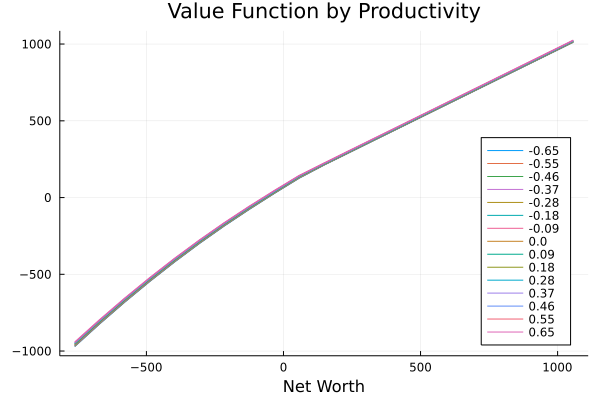
\includegraphics[scale = 0.5]{vf.png}
\end{center}
\end{frame}

\begin{frame}
\begin{center}
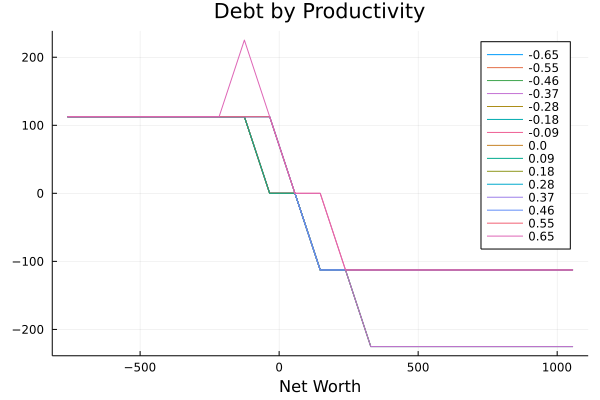
\includegraphics[scale = 0.5]{pf_b.png}
\end{center}
\end{frame}

\begin{frame}
\begin{center}
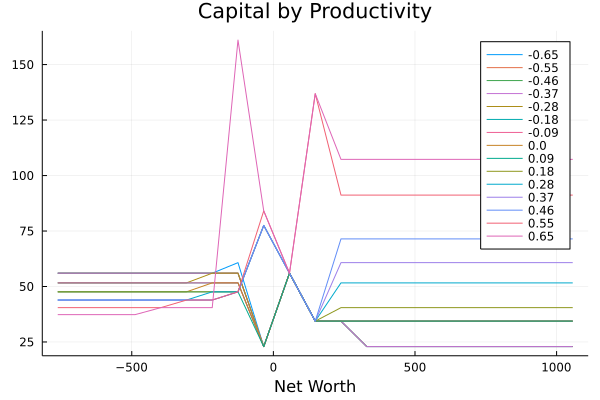
\includegraphics[scale = 0.5]{pf_k.png}
\end{center}
\end{frame}


\begin{frame}
\begin{center}
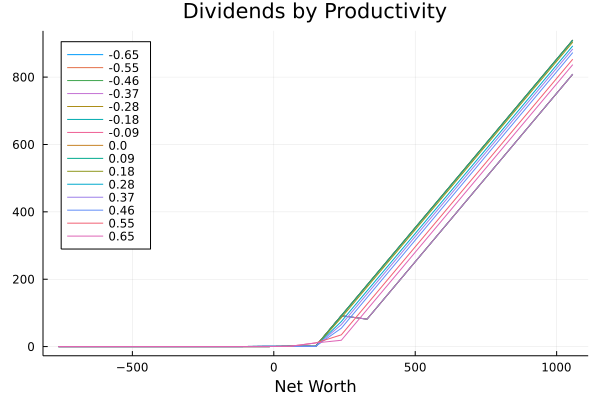
\includegraphics[scale = 0.5]{dividends.png}
\end{center}
\end{frame}

\begin{frame}
\begin{center}
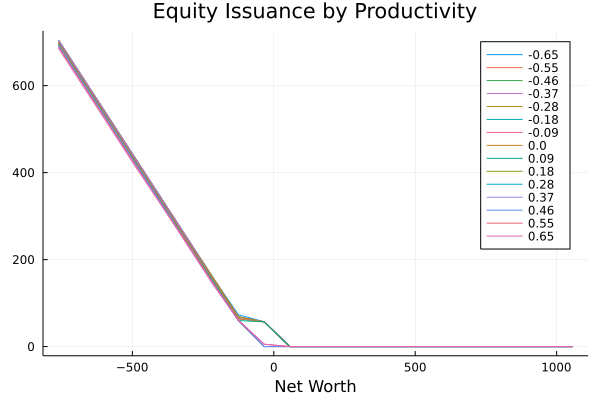
\includegraphics[scale = 0.5]{issuance.png}
\end{center}
\end{frame}

\begin{frame}
\begin{center}
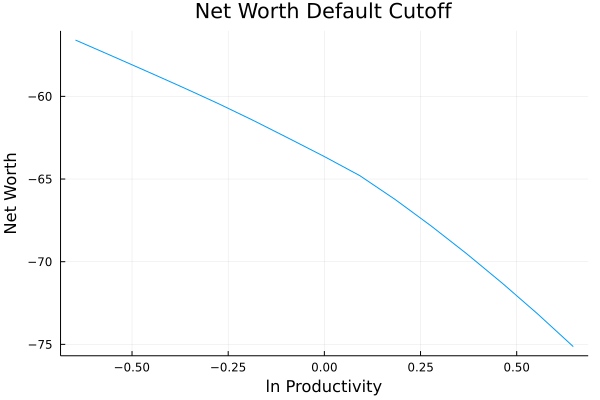
\includegraphics[scale = 0.5]{w_bar.png}
\end{center}
\end{frame}

\begin{frame}
\begin{center}
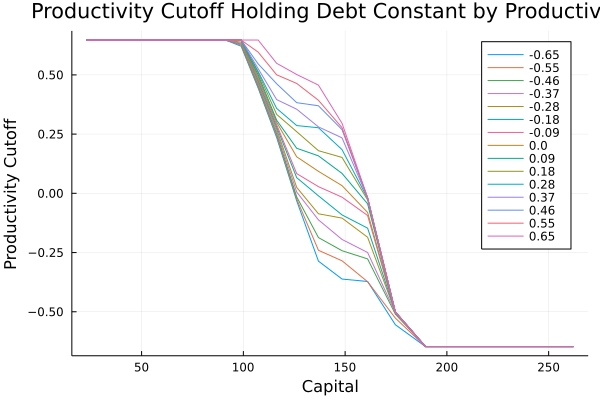
\includegraphics[scale = 0.5]{z_d.png}
\end{center}
\end{frame}

\begin{frame}
\begin{center}
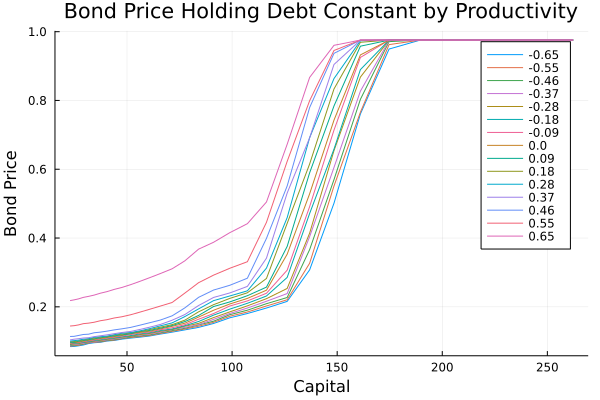
\includegraphics[scale = 0.5]{q.png}
\end{center}
\end{frame}

\begin{frame}
\frametitle{Data Replication}
\scriptsize
\begin{itemize}
\item I recomputed data moments for original period and recent period
\end{itemize}
\tiny
\begin{center}
\csvautotabular{table_replication_data.csv}
\end{center}
\scriptsize
\begin{itemize}
\item Comparing column 1 and column 2:
\begin{itemize}
\scriptsize
\item Var of equity iss./asset too small
\item Too much equity issuance and too high payout ratio
\item Cov. of inv. and lev. changes sign
\item Serial cor. of inc./assets too high and sd of shocks too high
\end{itemize}

\item Comparing column 2 and column 3:
\begin{itemize}
\scriptsize
\item Higher dividend variance $\implies$ change in $\phi$?
\item Lower mean debt-to-assets ratio and cov. of inv. and lev. changed sign $\implies$ change in $\xi$?
\end{itemize}
\end{itemize}
\end{frame}




\end{document}

